%% Creator: Inkscape inkscape 0.92.1, www.inkscape.org
%% PDF/EPS/PS + LaTeX output extension by Johan Engelen, 2010
%% Accompanies image file 'inout.pdf' (pdf, eps, ps)
%%
%% To include the image in your LaTeX document, write
%%   \input{<filename>.pdf_tex}
%%  instead of
%%   \includegraphics{<filename>.pdf}
%% To scale the image, write
%%   \def\svgwidth{<desired width>}
%%   \input{<filename>.pdf_tex}
%%  instead of
%%   \includegraphics[width=<desired width>]{<filename>.pdf}
%%
%% Images with a different path to the parent latex file can
%% be accessed with the `import' package (which may need to be
%% installed) using
%%   \usepackage{import}
%% in the preamble, and then including the image with
%%   \import{<path to file>}{<filename>.pdf_tex}
%% Alternatively, one can specify
%%   \graphicspath{{<path to file>/}}
%% 
%% For more information, please see info/svg-inkscape on CTAN:
%%   http://tug.ctan.org/tex-archive/info/svg-inkscape
%%
\begingroup%
  \makeatletter%
  \providecommand\color[2][]{%
    \errmessage{(Inkscape) Color is used for the text in Inkscape, but the package 'color.sty' is not loaded}%
    \renewcommand\color[2][]{}%
  }%
  \providecommand\transparent[1]{%
    \errmessage{(Inkscape) Transparency is used (non-zero) for the text in Inkscape, but the package 'transparent.sty' is not loaded}%
    \renewcommand\transparent[1]{}%
  }%
  \providecommand\rotatebox[2]{#2}%
  \ifx\svgwidth\undefined%
    \setlength{\unitlength}{429.98562493bp}%
    \ifx\svgscale\undefined%
      \relax%
    \else%
      \setlength{\unitlength}{\unitlength * \real{\svgscale}}%
    \fi%
  \else%
    \setlength{\unitlength}{\svgwidth}%
  \fi%
  \global\let\svgwidth\undefined%
  \global\let\svgscale\undefined%
  \makeatother%
  \begin{picture}(1,0.91389413)%
    \put(0,0){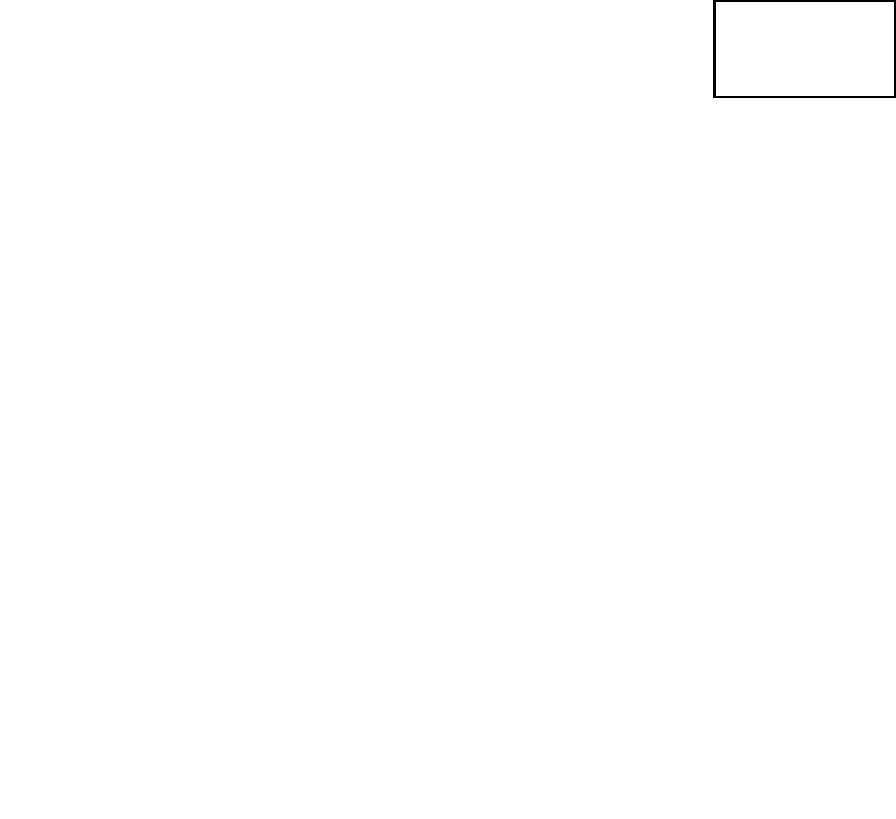
\includegraphics[width=\unitlength,page=1]{inout.pdf}}%
    \put(0.81,0.85){\color[rgb]{0,0,0}\makebox(0,0)[lb]{\smash{\footnotesize{obfuscator}}}}%
    \put(-0.01287918,1.11588507){\color[rgb]{0,0,0}\makebox(0,0)[lt]{\begin{minipage}{0.31663073\unitlength}\raggedright \end{minipage}}}%
    \put(0,0){\includegraphics[width=\unitlength,page=2]{inout.pdf}}%
    \put(0.025,0.845){\color[rgb]{0,0,0}\makebox(0,0)[lb]{\smash{SA}}}%
    \put(0.01702215,1.03365639){\color[rgb]{0,0,0}\makebox(0,0)[lt]{\begin{minipage}{0.86713864\unitlength}\raggedright \end{minipage}}}%
    \put(-0.13497628,1.42984905){\color[rgb]{0,0,0}\makebox(0,0)[lt]{\begin{minipage}{0.91946603\unitlength}\raggedright \end{minipage}}}%
    \put(0,0){\includegraphics[width=\unitlength,page=3]{inout.pdf}}%
    \put(0.18821872,0.826){\color[rgb]{0,0,0}\makebox(0,0)[lb]{\smash{\Large{*}}}}%
    \put(0.64190657,0.826){\color[rgb]{0,0,0}\makebox(0,0)[lb]{\smash{\Large{*}}}}%
    \put(0.29305761,0.826){\color[rgb]{0,0,0}\makebox(0,0)[lb]{\smash{\Large{*}}}}%
    \put(0,0){\includegraphics[width=\unitlength,page=4]{inout.pdf}}%
    \put(0.45370615,0.683){\color[rgb]{0,0,0}\makebox(0,0)[lb]{\smash{$\ts[2]$}}}%
    \put(0.24377396,0.683){\color[rgb]{0,0,0}\makebox(0,0)[lb]{\smash{$\ts[1]$}}}%
    \put(0,0){\includegraphics[width=\unitlength,page=5]{inout.pdf}}%
    \put(0.8676,0.69488612){\color[rgb]{0,0,0}\rotatebox{-90}{\makebox(0,0)[lb]{\smash{\Large{*}}}}}%
    \put(0.8676,0.26562168){\color[rgb]{0,0,0}\rotatebox{-90}{\makebox(0,0)[lb]{\smash{\Large{*}}}}}%
    \put(0.8676,0.48888206){\color[rgb]{0,0,0}\rotatebox{-90}{\makebox(0,0)[lb]{\smash{\Large{*}}}}}%
    \put(0,0){\includegraphics[width=\unitlength,page=6]{inout.pdf}}%
    \put(0.727,0.365){\color[rgb]{0,0,0}{\makebox(0,0)[lb]{\smash{$\hts[2]$}}}}%
    \put(0.727,0.575){\color[rgb]{0,0,0}{\makebox(0,0)[lb]{\smash{$\hts[1]$}}}}%
    \put(0,0){\includegraphics[width=\unitlength,page=7]{inout.pdf}}%
    \put(0.855,0.04){\color[rgb]{0,0,0}\makebox(0,0)[lb]{\smash{ESP}}}%
  \end{picture}%
\endgroup%
